\documentclass[aspectratio=169,xcolor={dvipsnames}]{beamer}

% Use UNIL theme
\usetheme{UNIL}

% Required packages
\usepackage{tikz}
\usepackage{listings}
\usepackage{array}
\usepackage{booktabs}
\usepackage{multirow}
\usepackage{amsmath}
\usepackage{amssymb}
\usepackage{subcaption}
\usepackage{pgfplots}

% TikZ libraries for diagrams
\usetikzlibrary{shapes,arrows,positioning,calc,fit,backgrounds,decorations.pathreplacing}

% PGFPlots version
\pgfplotsset{compat=1.17}

% Code listing style
\lstset{
    basicstyle=\ttfamily\small,
    keywordstyle=\color{blue},
    commentstyle=\color{gray},
    stringstyle=\color{red},
    showstringspaces=false,
    breaklines=true,
    frame=single,
    numbers=left,
    numberstyle=\tiny\color{gray},
    xleftmargin=2.5em,
    framexleftmargin=2.2em
}

% Define custom colors
\definecolor{codegreen}{rgb}{0,0.6,0}
\definecolor{codegray}{rgb}{0.5,0.5,0.5}
\definecolor{codepurple}{rgb}{0.58,0,0.82}
\definecolor{backcolour}{rgb}{0.95,0.95,0.92}

% Title information
\title{An Introduction to Parallel Computing}
\subtitle{\Large Foundations of High-Performance Computing (HPC)}
\author{Flavio Calvo \\ \emph{Université de Lausanne}}
\date{February 3-4, 2026}

\begin{document}

% Title slide
\begin{frame}[plain]
    \titlepage
\end{frame}

% Table of contents
\begin{frame}{Course Overview}
    \tableofcontents
\end{frame}

%%%%%%%%%%%%%%%%%%%%%%%%%%%%%%%%%%%%%%%%%%%%%%%%%%%%%%%%%%%%%%%%%%%%%%%%%%
\section{Demystifying HPC Hardware}
%%%%%%%%%%%%%%%%%%%%%%%%%%%%%%%%%%%%%%%%%%%%%%%%%%%%%%%%%%%%%%%%%%%%%%%%%%

\begin{frame}{What is High-Performance Computing?}
    \begin{itemize}
        \item \textbf{High-Performance Computing (HPC)}: Using supercomputers and parallel processing techniques to solve complex computational problems
        \item \textbf{Goals:}
        \begin{itemize}
            \item Solve problems faster (reduced time to solution)
            \item Solve larger problems (increased problem size)
            \item Solve more problems simultaneously (increased throughput)
        \end{itemize}
        \item \textbf{Applications:}
        \begin{itemize}
            \item Weather forecasting and climate modeling
            \item Molecular dynamics and drug discovery
            \item Computational fluid dynamics
            \item Machine learning and AI
            \item Genomics and bioinformatics
        \end{itemize}
    \end{itemize}
\end{frame}

\begin{frame}{What is Parallel Computing?}
    \begin{itemize}
        \item \textbf{Parallel Computing}: Performing multiple operations at the same time
        \item A broad concept encompassing various forms of simultaneous computation
        \item \textbf{Core Idea:}
        \begin{itemize}
            \item Break down a task into smaller tasks
            \item Execute these smaller tasks simultaneously
            \item Combine results to get the final solution
        \end{itemize}
    \end{itemize}
\end{frame}

\begin{frame}{CPU Architecture Basics}
	\footnotesize
    \begin{columns}[T]
        \begin{column}{0.5\textwidth}
            \textbf{Key Components:}
            \begin{itemize}
                \item \textbf{CPU (Central Processing Unit)}: The main processor chip
                \item \textbf{Core}: An independent processing unit within a CPU
                \item \textbf{Socket}: Physical connector for a CPU on the motherboard
                \item \textbf{Thread}: Virtual core via hyperthreading/SMT
            \end{itemize}
        \end{column}
        \begin{column}{0.5\textwidth}
			\centering\vspace{2.5em}
			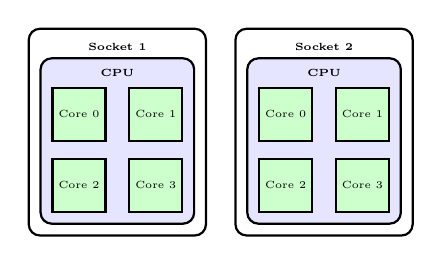
\begin{tikzpicture}[scale=0.75, every node/.style={scale=0.75}]
				% Socket 1
				\draw[thick, rounded corners] (0,0) rectangle (3,3.5);
				\node at (1.5, 3.2) {\textbf{\tiny Socket 1}};

				% CPU 1
				\draw[thick, rounded corners, fill=blue!10] (0.2,0.2) rectangle (2.8,3);
				\node at (1.5, 2.75) {\textbf{\tiny CPU}};

				% Cores in Socket 1 (wider boxes, centered)
				\draw[thick, fill=green!20] (0.4,1.6) rectangle (1.3,2.5);
				\node at (0.85, 2.05) {\tiny Core 0};

				\draw[thick, fill=green!20] (1.7,1.6) rectangle (2.6,2.5);
				\node at (2.15, 2.05) {\tiny Core 1};

				\draw[thick, fill=green!20] (0.4,0.4) rectangle (1.3,1.3);
				\node at (0.85, 0.85) {\tiny Core 2};

				\draw[thick, fill=green!20] (1.7,0.4) rectangle (2.6,1.3);
				\node at (2.15, 0.85) {\tiny Core 3};

				% Socket 2
				\draw[thick, rounded corners] (3.5,0) rectangle (6.5,3.5);
				\node at (5, 3.2) {\textbf{\tiny Socket 2}};

				% CPU 2
				\draw[thick, rounded corners, fill=blue!10] (3.7,0.2) rectangle (6.3,3);
				\node at (5, 2.75) {\textbf{\tiny CPU}};

				% Cores in Socket 2 (wider boxes, centered)
				\draw[thick, fill=green!20] (3.9,1.6) rectangle (4.8,2.5);
				\node at (4.35, 2.05) {\tiny Core 0};

				\draw[thick, fill=green!20] (5.2,1.6) rectangle (6.1,2.5);
				\node at (5.65, 2.05) {\tiny Core 1};

				\draw[thick, fill=green!20] (3.9,0.4) rectangle (4.8,1.3);
				\node at (4.35, 0.85) {\tiny Core 2};

				\draw[thick, fill=green!20] (5.2,0.4) rectangle (6.1,1.3);
				\node at (5.65, 0.85) {\tiny Core 3};
			\end{tikzpicture}
        \end{column}
    \end{columns}
    \vskip1em
    \textbf{Example:} A dual-socket server with 2 CPUs × 4 cores/CPU = 8 cores total
\end{frame}

\begin{frame}{Why Multiprocessing?}
	\footnotesize
	\begin{columns}[T]
		\begin{column}{0.5\textwidth}
			\textbf{Serial Computing Limitations:}
			\begin{itemize}
				\item CPU clock speeds plateaued (\textasciitilde2005)
				\item Physical limits (power, heat)
				\item Need for faster solutions
			\end{itemize}
			\vskip1em
			\textbf{Solution: Parallelism}
			\begin{itemize}
				\item Use multiple cores simultaneously
				\item Divide work among processors
				\item Reduce time to solution
			\end{itemize}
		\end{column}
		\begin{column}{0.5\textwidth}
			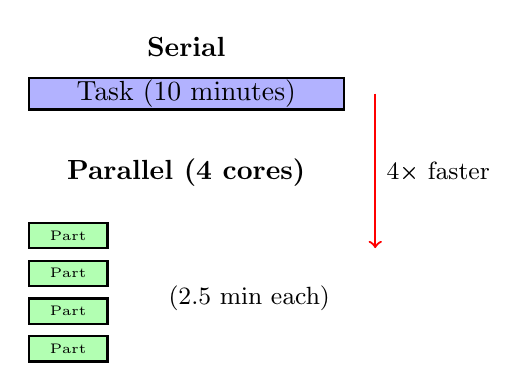
\begin{tikzpicture}[scale=0.8]
				% Serial execution
				\node at (2.5, 5) {\textbf{Serial}};
				\draw[thick, fill=blue!30] (0,4) rectangle (5,4.5);
				\node at (2.5, 4.25) {Task (10 minutes)};

				% Parallel execution
				\node at (2.5, 3) {\textbf{Parallel (4 cores)}};
				\foreach \y in {0,0.6,1.2,1.8} {
					\draw[thick, fill=green!30] (0,\y) rectangle (1.25,\y+0.4);
					\node at (0.625, \y+0.2) {\tiny Part};
				}
				\node at (3.5, 1) {\small (2.5 min each)};

				% Speedup arrow
				\draw[->, thick, red] (5.5, 4.25) -- (5.5, 1.8);
				\node at (6.5, 3) {\small 4× faster};
			\end{tikzpicture}
			\vskip0.3em
			\small
			\textbf{Note:} Ideal speedup is rarely achieved due to overhead and serial portions
		\end{column}
	\end{columns}
\end{frame}

\begin{frame}{Memory Hierarchy}
    \begin{columns}[T]
        \begin{column}{0.55\textwidth}
            \textbf{Levels of Memory:}
            \begin{enumerate}
                \item \textbf{Registers}: Fastest, smallest (bytes)
                \item \textbf{L1 Cache}: Very fast, per-core (KB)
                \item \textbf{L2 Cache}: Fast, per-core (KB)
                \item \textbf{L3 Cache}: Shared, per-CPU (MB)
                \item \textbf{Main Memory (RAM)}: Large (GB)
                \item \textbf{Storage (Disk)}: Largest, slowest (TB)
            \end{enumerate}
            \vskip0.5em
            \textbf{Key Principle:} Faster memory is smaller and more expensive
        \end{column}
        \begin{column}{0.45\textwidth}
            \centering
            \vspace{1em}
			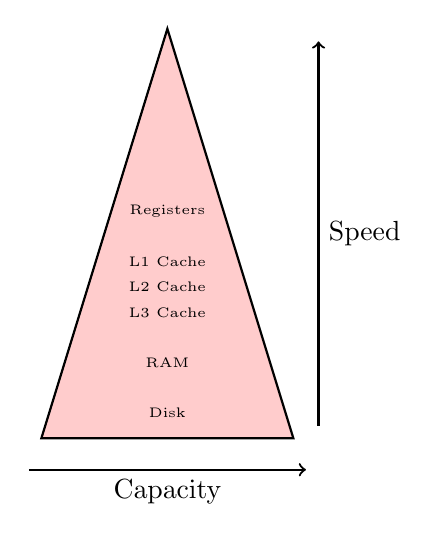
\begin{tikzpicture}[scale=0.8]
				% Triangle representing hierarchy - extended higher
				\draw[thick, fill=red! 20] (0,0) -- (4,0) -- (2,6.5) -- cycle;

				% Labels - sorted from fastest (top) to slowest (bottom)
				% Top part left empty (too narrow)
				\node at (2, 3.6) {\tiny Registers};
				\node at (2, 2.8) {\tiny L1 Cache};
				\node at (2, 2.4) {\tiny L2 Cache};
				\node at (2, 2.0) {\tiny L3 Cache};
				\node at (2, 1.2) {\tiny RAM};
				\node at (2, 0.4) {\tiny Disk};

				% Arrows for speed (bottom to top = slowest to fastest)
				\draw[->, thick] (4.4, 0.2) -- (4.4, 6.3) node[midway, right] {Speed};
				% Capacity arrow outside the triangle
				\draw[->, thick] (-0.2, -0.5) -- (4.2, -0.5) node[midway, below] {Capacity};
			\end{tikzpicture}
        \end{column}
    \end{columns}
\end{frame}

\begin{frame}{Shared vs Distributed Memory}
    \begin{columns}[T]
        \begin{column}{0.5\textwidth}
            \textbf{Shared Memory:}
            \begin{itemize}
                \item All cores access same RAM
                \item Fast communication
                \item Limited scalability
                \item Example: Multi-core CPU
            \end{itemize}
            \vspace{1em}
            \centering
            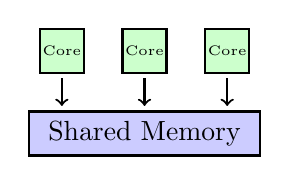
\begin{tikzpicture}[scale=0.7]
                % Cores
                \foreach \x in {0,1.5,3} {
                    \draw[thick, fill=green!20] (\x,2) rectangle (\x+0.8,2.8);
                    \node at (\x+0.4, 2.4) {\tiny Core};
                }
                % Shared memory - wider box
                \draw[thick, fill=blue!20] (-0.2,0.5) rectangle (4.0,1.3);
                \node at (1.9, 0.9) {Shared Memory};
                % Arrows
                \foreach \x in {0.4,1.9,3.4} {
                    \draw[->, thick] (\x, 1.9) -- (\x, 1.4);
                }
            \end{tikzpicture}
        \end{column}
        \begin{column}{0.5\textwidth}
            \textbf{Distributed Memory:}
            \begin{itemize}
                \item Each node has its own RAM
                \item Explicit data transfer (MPI)
                \item Highly scalable
                \item Example: HPC cluster
            \end{itemize}
            \vspace{1em}
            \centering
            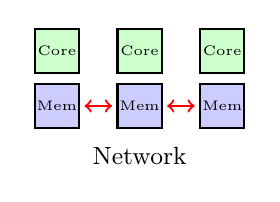
\begin{tikzpicture}[scale=0.7]
                % Node 1
                \draw[thick, fill=green!20] (0,2.5) rectangle (0.8,3.3);
                \node at (0.4, 2.9) {\tiny Core};
                \draw[thick, fill=blue!20] (0,1.5) rectangle (0.8,2.3);
                \node at (0.4, 1.9) {\tiny Mem};

                % Node 2
                \draw[thick, fill=green!20] (1.5,2.5) rectangle (2.3,3.3);
                \node at (1.9, 2.9) {\tiny Core};
                \draw[thick, fill=blue!20] (1.5,1.5) rectangle (2.3,2.3);
                \node at (1.9, 1.9) {\tiny Mem};

                % Node 3
                \draw[thick, fill=green!20] (3,2.5) rectangle (3.8,3.3);
                \node at (3.4, 2.9) {\tiny Core};
                \draw[thick, fill=blue!20] (3,1.5) rectangle (3.8,2.3);
                \node at (3.4, 1.9) {\tiny Mem};

                % Network
                \draw[thick, <->, red] (0.9, 1.9) -- (1.4, 1.9);
                \draw[thick, <->, red] (2.4, 1.9) -- (2.9, 1.9);
                \node at (1.9, 1.0) {\small Network};
            \end{tikzpicture}
        \end{column}
    \end{columns}
\end{frame}

\begin{frame}{Compute Nodes in a HPC Cluster}
    \centering
    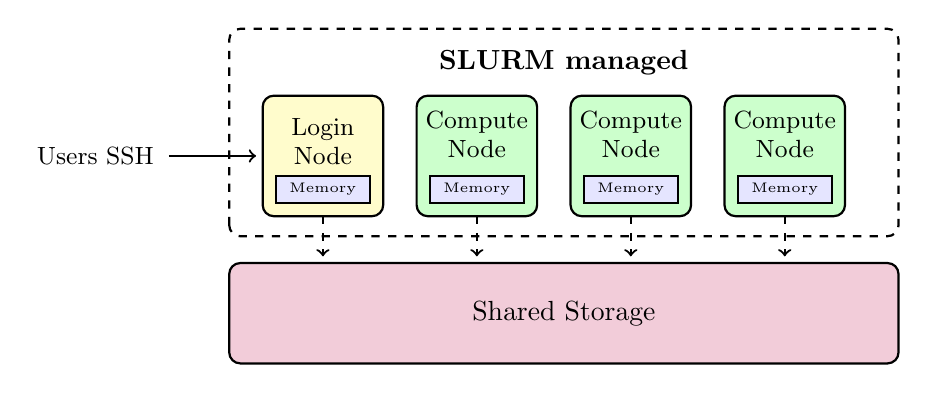
\begin{tikzpicture}[scale=0.85]
        % Big box for SLURM managed
        \draw[thick, rounded corners, dashed] (-0.5,1.9) rectangle (9.5,5.0);
        \node at (4.5, 4.5) {\textbf{SLURM managed}};

        % Login node (at same level as compute nodes)
        \draw[thick, fill=yellow!20, rounded corners] (0,2.2) rectangle (1.8,4);
        \node at (0.9, 3.5) {\small Login};
        \node at (0.9, 3.1) {\small Node};
        \draw[thick, fill=blue!10] (0.2,2.4) rectangle (1.6,2.8);
        \node at (0.9, 2.6) {\tiny Memory};

        % Compute nodes
        \foreach \x in {2.3,4.6,6.9} {
            \draw[thick, fill=green!20, rounded corners] (\x,2.2) rectangle (\x+1.8,4);
            \node at (\x+0.9, 3.6) {\small Compute};
            \node at (\x+0.9, 3.2) {\small Node};
            \draw[thick, fill=blue!10] (\x+0.2,2.4) rectangle (\x+1.6,2.8);
            \node at (\x+0.9, 2.6) {\tiny Memory};
        }

        % Storage - much wider
        \draw[thick, fill=purple!20, rounded corners] (-0.5,0) rectangle (9.5,1.5);
        \node at (4.5, 0.75) {Shared Storage};

        % Storage connections
        \foreach \x in {0.9,3.2,5.5,7.8} {
            \draw[->, thick, dashed] (\x, 2.2) -- (\x, 1.6);
        }

        % Users SSH arrow
        \node at (-2.5, 3.1) {\small Users SSH};
        \draw[->, thick] (-1.4, 3.1) -- (-0.1, 3.1);
    \end{tikzpicture}

    \vskip0.5em
    \textbf{Workflow:} Users connect to the login node $\rightarrow$ Submit jobs to SLURM $\rightarrow$ Jobs run on compute nodes
\end{frame}

\begin{frame}{SLURM Terminology: CPUs vs Tasks}
    \footnotesize
    {
    \begin{columns}[T]
        \begin{column}{0.5\textwidth}
            \textbf{Key Terms:}
            \begin{itemize}
                \item \textbf{Node}: A single computer in the cluster
                \item \textbf{CPU}: In SLURM, often means a "core"
                \item \textbf{Task}: A process (instance of a program)
                \item \textbf{CPUs per task}: Cores available to each task
            \end{itemize}
            \vskip0.5em
            \textbf{Important:} 
            \begin{itemize}
                \item SLURM's "cpu" ≠ physical CPU
                \item Usually means a core or hardware thread
                \item Check your cluster's definition!
            \end{itemize}
        \end{column}
        \begin{column}{0.5\textwidth}
            \textbf{Example Configurations:}
            \vskip0.5em
            \begin{tabular}{lcc}
                \toprule
                \textbf{Config} & \textbf{Tasks} & \textbf{CPUs/Task} \\
                \midrule
                Serial & 1 & 1 \\
                Multi-threaded & 1 & 16 \\
                MPI (distributed) & 32 & 1 \\
                Hybrid & 4 & 8 \\
                \bottomrule
            \end{tabular}
            \vskip0.5em
            \textbf{Resource Calculation:}
            \begin{itemize}
                \item Total CPUs = Tasks × CPUs per task
                \item Example: 4 tasks × 8 CPUs = 32 cores
            \end{itemize}
        \end{column}
    \end{columns}
    }
\end{frame}

\begin{frame}{Understanding Resource Allocation}
    \centering
    \vspace{0.5em}
	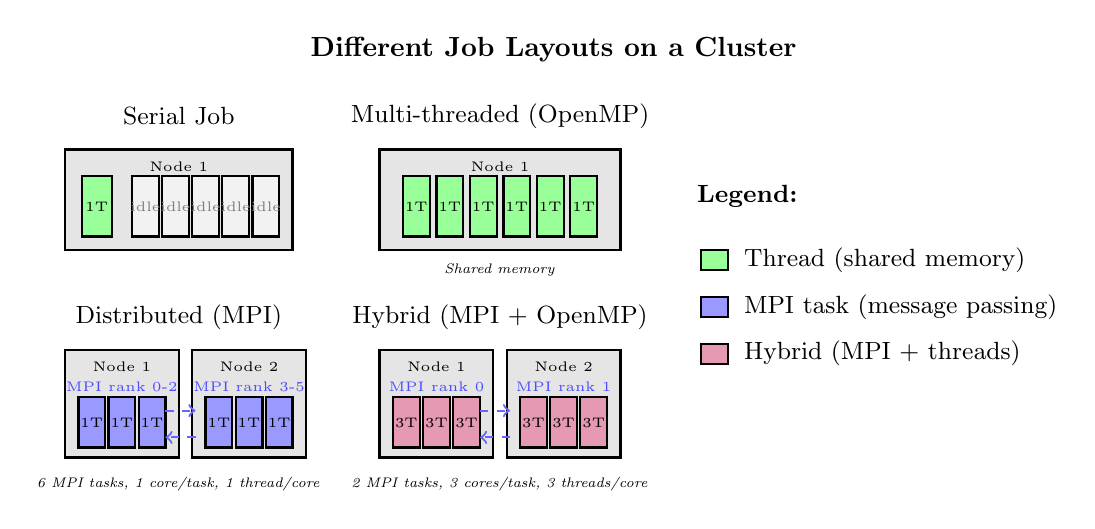
\begin{tikzpicture}[scale=0.85]
		% Title (centered)
		\node at (7.8, 6.8) {\textbf{Different Job Layouts on a Cluster}};

		% Single Node - Serial Job
		\node at (2.2, 5.8) {\small Serial Job};
		\draw[thick, fill=gray!20] (0.5,3.8) rectangle (3.9,5.3);
		\node at (2.2, 5.05) {\tiny Node 1};
		\draw[thick, fill=green!40] (0.75,4.0) rectangle (1.2,4.9);
		\node at (0.975, 4.45) {\tiny 1T};
		\foreach \x in {1.5,1.95,2.4,2.85,3.3} {
			\draw[thick, fill=gray!10] (\x,4.0) rectangle (\x+0.4,4.9);
			\node[gray] at (\x+0.2, 4.45) {\tiny idle};
		}

		% Multi-threaded Job (OpenMP) - now properly centered
		\node at (7, 5.8) {\small Multi-threaded (OpenMP)};
		\draw[thick, fill=gray!20] (5.2,3.8) rectangle (8.8,5.3);
		\node at (7, 5.05) {\tiny Node 1};
		\foreach \x in {5.55,6.05,6.55,7.05,7.55,8.05} {
			\draw[thick, fill=green!40] (\x,4.0) rectangle (\x+0.4,4.9);
			\node at (\x+0.2, 4.45) {\tiny 1T};
		}
		\node at (7, 3.5) {\tiny\textit{Shared memory}};

		% Distributed MPI Job
		\node at (2.2, 2.8) {\small Distributed (MPI)};
		\node at (2.2, 0.3) {\tiny\textit{6 MPI tasks, 1 core/task, 1 thread/core}};
		% Node 1 - MPI ranks 0-2
		\draw[thick, fill=gray!20] (0.5,0.7) rectangle (2.2,2.3);
		\node at (1.35, 2.05) {\tiny Node 1};
		\node at (1.35, 1.75) {\tiny\textcolor{blue!70}{MPI rank 0-2}};
		\foreach \x in {0.7,1.15,1.6} {
			\draw[thick, fill=blue!40] (\x,0.85) rectangle (\x+0.4,1.6);
			\node at (\x+0.2, 1.225) {\tiny 1T};
		}
		% Node 2 - MPI ranks 3-5
		\draw[thick, fill=gray!20] (2.4,0.7) rectangle (4.1,2.3);
		\node at (3.25, 2.05) {\tiny Node 2};
		\node at (3.25, 1.75) {\tiny\textcolor{blue!70}{MPI rank 3-5}};
		\foreach \x in {2.6,3.05,3.5} {
			\draw[thick, fill=blue!40] (\x,0.85) rectangle (\x+0.4,1.6);
			\node at (\x+0.2, 1.225) {\tiny 1T};
		}

		% Hybrid Job (MPI + OpenMP)
		\node at (7, 2.8) {\small Hybrid (MPI + OpenMP)};
		\node at (7, 0.3) {\tiny\textit{2 MPI tasks, 3 cores/task, 3 threads/core}};
		% Node 1 - MPI rank 0
		\draw[thick, fill=gray!20] (5.2,0.7) rectangle (6.9,2.3);
		\node at (6.05, 2.05) {\tiny Node 1};
		\node at (6.05, 1.75) {\tiny\textcolor{blue!70}{MPI rank 0}};
		\foreach \x in {5.4,5.85,6.3} {
			\draw[thick, fill=purple!40] (\x,0.85) rectangle (\x+0.4,1.6);
			\node at (\x+0.2, 1.225) {\tiny 3T};
		}
		% Node 2 - MPI rank 1
		\draw[thick, fill=gray!20] (7.1,0.7) rectangle (8.8,2.3);
		\node at (7.95, 2.05) {\tiny Node 2};
		\node at (7.95, 1.75) {\tiny\textcolor{blue!70}{MPI rank 1}};
		\foreach \x in {7.3,7.75,8.2} {
			\draw[thick, fill=purple!40] (\x,0.85) rectangle (\x+0.4,1.6);
			\node at (\x+0.2, 1.225) {\tiny 3T};
		}

		% Enhanced Legend with more spacing
		\node[anchor=west] at (9.8, 4.6) {\small\textbf{Legend:}};

		\draw[thick, fill=green!40] (10,3.5) rectangle (10.4,3.8);
		\node[anchor=west] at (10.5, 3.65) {\small Thread (shared memory)};

		\draw[thick, fill=blue!40] (10,2.8) rectangle (10.4,3.1);
		\node[anchor=west] at (10.5, 2.95) {\small MPI task (message passing)};

		\draw[thick, fill=purple!40] (10,2.1) rectangle (10.4,2.4);
		\node[anchor=west] at (10.5, 2.25) {\small Hybrid (MPI + threads)};

		% Add communication arrows for MPI
		\draw[->, thick, blue!60, dashed] (2.0, 1.4) -- (2.45, 1.4);
		\draw[->, thick, blue!60, dashed] (2.45, 1.0) -- (2.0, 1.0);
		\draw[->, thick, blue!60, dashed] (6.7, 1.4) -- (7.15, 1.4);
		\draw[->, thick, blue!60, dashed] (7.15, 1.0) -- (6.7, 1.0);
	\end{tikzpicture}
\end{frame}

%%%%%%%%%%%%%%%%%%%%%%%%%%%%%%%%%%%%%%%%%%%%%%%%%%%%%%%%%%%%%%%%%%%%%%%%%%
\section{Understanding Parallelism}
%%%%%%%%%%%%%%%%%%%%%%%%%%%%%%%%%%%%%%%%%%%%%%%%%%%%%%%%%%%%%%%%%%%%%%%%%%

\begin{frame}{Levels of Parallelism - Part 1}
    \begin{enumerate}
        \item \textbf{Instruction-Level Parallelism (ILP)}
        \begin{itemize}
            \item Pipelining and out-of-order execution
            \item Automatic (hardware-level)
            \item Not programmable by users
        \end{itemize}
        \vskip1em

        \item \textbf{Vectorization (SIMD)}
        \begin{itemize}
            \item Single Instruction, Multiple Data
            \item Process multiple data elements simultaneously
            \item Compiler can auto-vectorize or use intrinsics
        \end{itemize}
    \end{enumerate}
\end{frame}

\begin{frame}{Levels of Parallelism - Part 2}
    \begin{enumerate}
        \setcounter{enumi}{2}
        \item \textbf{Thread-Level Parallelism (Shared Memory)}
        \begin{itemize}
            \item Multiple threads on same node
            \item OpenMP, pthreads, threading libraries
            \item Access shared memory space
        \end{itemize}
        \vskip1em

        \item \textbf{Process-Level Parallelism (Distributed Memory)}
        \begin{itemize}
            \item Multiple processes across nodes
            \item MPI (Message Passing Interface)
            \item Explicit communication between processes
        \end{itemize}
    \end{enumerate}
\end{frame}

\begin{frame}{Parallelism Hierarchy}
    \begin{columns}[T]
        \begin{column}{0.55\textwidth}
            \textbf{Levels of Parallelism:}
            \begin{enumerate}
                \item \textbf{ILP}: Automatic, hardware-level (ns)
                \item \textbf{SIMD}: Vectorization, per-core (ns)
                \item \textbf{Threads}: Shared memory, per-node (µs)
                \item \textbf{Processes}: Distributed memory, MPI (ms)
                \item \textbf{Accelerators}: GPUs, FPGAs (massive parallelism)
            \end{enumerate}
            \vskip0.5em
            \textbf{Key Principle:} Higher levels offer more parallelism but require more explicit programming
        \end{column}
        \begin{column}{0.45\textwidth}
            \centering
            \vspace{0.5em}
			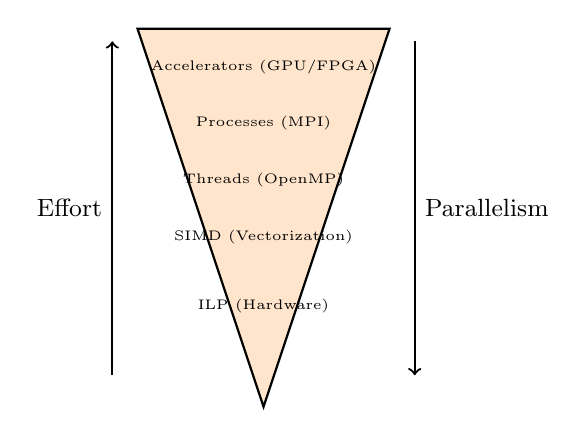
\begin{tikzpicture}[scale=0.8]
				% Inverted triangle (pyramid) - wide at top, narrow at bottom
				\draw[thick, fill=orange!20] (0,6) -- (4,6) -- (2,0) -- cycle;

				% Labels - from most parallelism (top) to least (bottom)
				\node at (2, 5.4) {\tiny Accelerators (GPU/FPGA)};
				\node at (2, 4.5) {\tiny Processes (MPI)};
				\node at (2, 3.6) {\tiny Threads (OpenMP)};
				\node at (2, 2.7) {\tiny SIMD (Vectorization)};
				\node at (2, 1.6) {\tiny ILP (Hardware)};

				% Arrow for parallelism potential (top to bottom = more to less)
				\draw[<-, thick] (4.4, 0.5) -- (4.4, 5.8) node[midway, right, align=left] {\small Parallelism};
				% Arrow for programmer effort
				\draw[->, thick] (-0.4, 0.5) -- (-0.4, 5.8) node[midway, left, align=right] {\small Effort};
			\end{tikzpicture}
        \end{column}
    \end{columns}
\end{frame}

\begin{frame}{Accelerators: GPUs and Beyond}
	\footnotesize
    \begin{columns}[T]
        \begin{column}{0.5\textwidth}
            \textbf{GPU Computing:}
            \begin{itemize}
                \item Thousands of simple cores
                \item Massive data parallelism
                \item Best for: matrix ops, deep learning, simulations
            \end{itemize}
            \vskip0.5em
            \textbf{Programming Models:}
            \begin{itemize}
                \item \textbf{CUDA}: NVIDIA GPUs (most common)
                \item \textbf{ROCm/HIP}: AMD GPUs
                \item \textbf{OpenCL}: Cross-platform
                \item \textbf{SYCL}: Modern C++ approach
            \end{itemize}
            \vskip0.5em
            \textbf{High-Level Libraries:}
            \begin{itemize}
                \item PyTorch, TensorFlow (ML)
                \item CuPy, JAX (array computing)
                \item RAPIDS (data science)
            \end{itemize}
        \end{column}
        \begin{column}{0.5\textwidth}
            \centering
            \vspace{1em}
            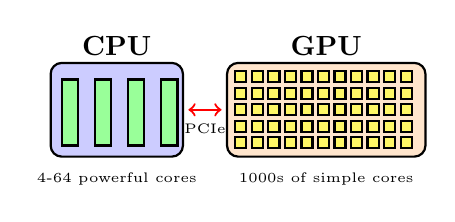
\begin{tikzpicture}[scale=0.7]
                % CPU side
                \node at (1.2, 4.5) {\textbf{CPU}};
                \draw[thick, fill=blue!20, rounded corners] (0,2.5) rectangle (2.4,4.2);
                \foreach \x in {0.2,0.8,1.4,2.0} {
                    \draw[thick, fill=green!40] (\x,2.7) rectangle (\x+0.3,3.9);
                }
                \node at (1.2, 2.1) {\tiny 4-64 powerful cores};

                % GPU side
                \node at (5, 4.5) {\textbf{GPU}};
                \draw[thick, fill=orange!20, rounded corners] (3.2,2.5) rectangle (6.8,4.2);
                \foreach \x in {3.35,3.65,3.95,4.25,4.55,4.85,5.15,5.45,5.75,6.05,6.35} {
                    \foreach \y in {2.65,2.95,3.25,3.55,3.85} {
                        \draw[thick, fill=yellow!60] (\x,\y) rectangle (\x+0.2,\y+0.2);
                    }
                }
                \node at (5, 2.1) {\tiny 1000s of simple cores};

                % Arrow between
                \draw[<->, thick, red] (2.5, 3.35) -- (3.1, 3.35);
                \node at (2.8, 3.0) {\tiny PCIe};
            \end{tikzpicture}
            \vskip0.5em
            \textbf{SLURM GPU Allocation:}
            \begin{itemize}
                \item \texttt{--gres=gpu:1} (1 GPU)
                \item \texttt{--gres=gpu:a100:2} (2 A100s)
                \item \texttt{--partition=gpu}
            \end{itemize}
        \end{column}
    \end{columns}
\end{frame}

\begin{frame}{Vectorization (SIMD)}
	\footnotesize
    \begin{columns}[T]
        \begin{column}{0.5\textwidth}
            \textbf{Concept:} Apply same operation to multiple data elements simultaneously
            \vskip1em
            \textbf{Example: Vector Addition}
            \begin{align*}
                C[0:3] = A[0:3] + B[0:3]
            \end{align*}
            \vskip0.5em
            %\centering
			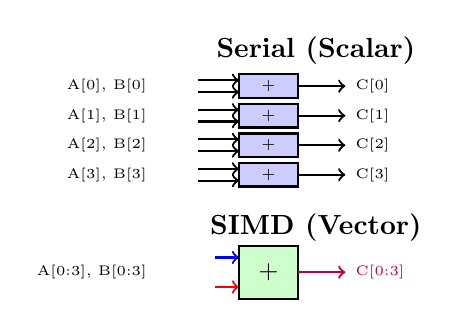
\begin{tikzpicture}[scale=0.75]
				% Serial
				\node at (2.5, 5.5) {\textbf{Serial (Scalar)}};
				\foreach \y/\n in {5/0,4.5/1,4/2,3.5/3} {
					\node[left] at (-0.2,\y-0.1) {\tiny A[\n], B[\n]};
					\draw[->, thick] (0.5,\y) -- (1.2,\y);
					\draw[->, thick] (0.5,\y-0.2) -- (1.2,\y-0.2);
					\draw[thick, fill=blue!20] (1.2,\y-0.3) rectangle (2.2,\y+0.1);
					\node at (1.7, \y-0.1) {\tiny +};
					\draw[->, thick] (2.2,\y-0.1) -- (3,\y-0.1) node[right] {\tiny C[\n]};
				}

				% SIMD
				\node at (2.5, 2.5) {\textbf{SIMD (Vector)}};
				\node[left] at (-0.2,1.75) {\tiny A[0:3], B[0:3]};
				\draw[->, thick, blue] (0.8,2) -- (1.2,2);
				\draw[->, thick, red] (0.8,1.5) -- (1.2,1.5);
				\draw[thick, fill=green!20] (1.2,1.3) rectangle (2.2,2.2);
				\node at (1.7, 1.75) {\small +};
				\draw[->, thick, purple] (2.2,1.75) -- (3,1.75) node[right] {\tiny C[0:3]};
			\end{tikzpicture}
        \end{column}
        \begin{column}{0.5\textwidth}
            \textbf{Without SIMD:}
		\begin{itemize}
			\item 4 separate additions
			\item 4 clock cycles
		\end{itemize}
		\vskip0.5em
		\textbf{With SIMD:}
		\begin{itemize}
			\item 1 vector addition
			\item 1 clock cycle
			\item 4× speedup!
		\end{itemize}
            \vskip0.5em
            \textbf{Modern CPUs:}
            \begin{itemize}
                \item AVX-512: 512-bit vectors
                \item Process 16 floats at once
            \end{itemize}
        \end{column}
    \end{columns}
\end{frame}

\begin{frame}[fragile]{Multi-Threading (Shared Memory)}
    \begin{columns}[T]
        \begin{column}{0.5\textwidth}
            \textbf{Thread-Level Parallelism:}
            \begin{itemize}
                \item Multiple threads in same process
                \item Share memory address space
                \item Lightweight context switching
                \item Common APIs: OpenMP, pthreads, C++ threads
            \end{itemize}
            \vskip1em
            \textbf{OpenMP Example:}
            \begin{lstlisting}[language=C, basicstyle=\tiny\ttfamily]
#pragma omp parallel for
for (int i = 0; i < N; i++) {
    c[i] = a[i] + b[i];
}
            \end{lstlisting}
        \end{column}
        \begin{column}{0.5\textwidth}
            \centering
            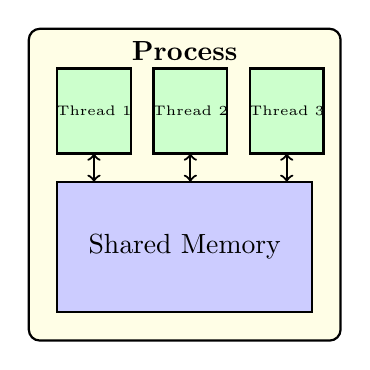
\begin{tikzpicture}[scale=0.72]
                % Process - with more spacing
                \draw[thick, rounded corners, fill=yellow!10] (0,0) rectangle (5.5,5.5);
                \node at (2.75, 5.1) {\textbf{Process}};

                % Threads - wider boxes
                \draw[thick, fill=green!20] (0.5,3.3) rectangle (1.8,4.8);
                \node at (1.15, 4.05) {\tiny Thread 1};

                \draw[thick, fill=green!20] (2.2,3.3) rectangle (3.5,4.8);
                \node at (2.85, 4.05) {\tiny Thread 2};

                \draw[thick, fill=green!20] (3.9,3.3) rectangle (5.2,4.8);
                \node at (4.55, 4.05) {\tiny Thread 3};

                % Shared memory
                \draw[thick, fill=blue!20] (0.5,0.5) rectangle (5,2.8);
                \node at (2.75, 1.65) {Shared Memory};

                % Arrows
                \draw[<->, thick] (1.15, 3.3) -- (1.15, 2.8);
                \draw[<->, thick] (2.85, 3.3) -- (2.85, 2.8);
                \draw[<->, thick] (4.55, 3.3) -- (4.55, 2.8);
            \end{tikzpicture}
            \vskip0.5em
            \textbf{Benefits:} Fast communication, easy data sharing
        \end{column}
    \end{columns}
\end{frame}

\begin{frame}{Message Passing (Distributed Memory)}
    \footnotesize
    \begin{columns}[T]
        \begin{column}{0.5\textwidth}
            \textbf{Message Passing Interface (MPI):}
            \begin{itemize}
                \item Multiple processes with separate memory
                \item Explicit communication via messages
                \item Scales across many nodes
                \item Standard library with many implementations
            \end{itemize}
            \vskip0.5em
            \textbf{Key Operations:}
            \begin{itemize}
                \item \texttt{MPI\_Send}: Send data
                \item \texttt{MPI\_Recv}: Receive data
                \item \texttt{MPI\_Bcast}: Broadcast to all
                \item \texttt{MPI\_Reduce}: Collect and combine
            \end{itemize}
        \end{column}
        \begin{column}{0.5\textwidth}
            \vspace{2em}
            \centering
            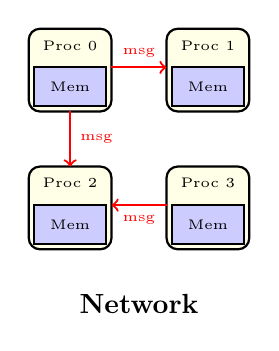
\begin{tikzpicture}[scale=0.7]
                % Process 0
                \draw[thick, rounded corners, fill=yellow!10] (0,4) rectangle (1.5,5.5);
                \node at (0.75, 5.2) {\tiny Proc 0};
                \draw[thick, fill=blue!20] (0.1,4.1) rectangle (1.4,4.8);
                \node at (0.75, 4.45) {\tiny Mem};

                % Process 1
                \draw[thick, rounded corners, fill=yellow!10] (2.5,4) rectangle (4,5.5);
                \node at (3.25, 5.2) {\tiny Proc 1};
                \draw[thick, fill=blue!20] (2.6,4.1) rectangle (3.9,4.8);
                \node at (3.25, 4.45) {\tiny Mem};

                % Process 2
                \draw[thick, rounded corners, fill=yellow!10] (0,1.5) rectangle (1.5,3);
                \node at (0.75, 2.7) {\tiny Proc 2};
                \draw[thick, fill=blue!20] (0.1,1.6) rectangle (1.4,2.3);
                \node at (0.75, 1.95) {\tiny Mem};

                % Process 3
                \draw[thick, rounded corners, fill=yellow!10] (2.5,1.5) rectangle (4,3);
                \node at (3.25, 2.7) {\tiny Proc 3};
                \draw[thick, fill=blue!20] (2.6,1.6) rectangle (3.9,2.3);
                \node at (3.25, 1.95) {\tiny Mem};

                % Communication arrows
                \draw[->, thick, red] (1.5, 4.8) -- (2.5, 4.8) node[midway, above] {\tiny msg};
                \draw[->, thick, red] (0.75, 4) -- (0.75, 3) node[midway, right] {\tiny msg};
                \draw[->, thick, red] (2.5, 2.3) -- (1.5, 2.3) node[midway, below] {\tiny msg};

                % Network
                \node at (2, 0.5) {\textbf{Network}};
            \end{tikzpicture}
            \vskip0.3em
            \textbf{Trade-off:} More complex but highly scalable
        \end{column}
    \end{columns}
\end{frame}

\begin{frame}{Hybrid Parallelization}
	\footnotesize
    \begin{columns}[T]
        \begin{column}{0.65\textwidth}
            \textbf{Combining MPI + OpenMP:}
            \begin{itemize}
                \item MPI for inter-node communication
                \item OpenMP for intra-node parallelism
                \item Best of both worlds
                \item Common in modern HPC applications
            \end{itemize}
            \vskip1em
            \textbf{Benefits:}
            \begin{itemize}
                \item Reduced message passing overhead
                \item Better memory utilization
                \item Improved scalability
                \item Flexible resource allocation
            \end{itemize}
        \end{column}
        \begin{column}{0.35\textwidth}
            \vspace{2em}
            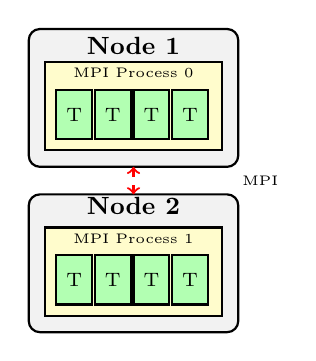
\begin{tikzpicture}[scale=0.7]
                % Node 1
                \draw[thick, rounded corners, fill=gray!10] (0,3) rectangle (3.8,5.5);
                \node at (1.9, 5.2) {\textbf{\small Node 1}};

                % MPI process 1
                \draw[thick, fill=yellow!20] (0.3,3.3) rectangle (3.5,4.9);
                \node at (1.9, 4.7) {\tiny MPI Process 0};

                % OpenMP threads - wider boxes
                \foreach \x in {0.5,1.2,1.9,2.6} {
                    \draw[thick, fill=green!30] (\x,3.5) rectangle (\x+0.65,4.4);
                    \node at (\x+0.325, 3.95) {\scriptsize T};
                }

                % Node 2
                \draw[thick, rounded corners, fill=gray!10] (0,0) rectangle (3.8,2.5);
                \node at (1.9, 2.3) {\textbf{\small Node 2}};

                % MPI process 2
                \draw[thick, fill=yellow!20] (0.3,0.3) rectangle (3.5,1.9);
                \node at (1.9, 1.7) {\tiny MPI Process 1};

                % OpenMP threads - wider boxes
                \foreach \x in {0.5,1.2,1.9,2.6} {
                    \draw[thick, fill=green!30] (\x,0.5) rectangle (\x+0.65,1.4);
                    \node at (\x+0.325, 0.95) {\scriptsize T};
                }

                % MPI communication
                \draw[<->, thick, red, dashed] (1.9, 3) -- (1.9, 2.5);
                \node at (4.2, 2.75) {\tiny MPI};
            \end{tikzpicture}
        \end{column}
    \end{columns}
    \vskip0.5em
    \textbf{Example:} 2 nodes × 4 threads = 8 total cores, but only 2 MPI processes
\end{frame}

\begin{frame}{Understanding Speed-Up}
	\footnotesize
    \begin{columns}[T]
        \begin{column}{0.5\textwidth}
            \textbf{Definition:}
            \begin{itemize}
                \item Speed-up measures how much faster a parallel program runs compared to serial
                \item Definition:
                \[
                S = \frac{T_{\text{serial}}}{T_{\text{parallel}}}
                \]
            \end{itemize}
            \vskip.1em
            \textbf{Efficiency:}
            \begin{itemize}
                \item Measures how well we use processors
                \item Definition:
                \[
                E = \frac{S}{N} = \frac{T_{\text{serial}}}{N \times T_{\text{parallel}}}
                \]
                \item Perfect efficiency: $E = 1$ (100\%)
                \item Typical: $E = 0.7-0.9$ (70-90\%)
            \end{itemize}
        \end{column}
        \begin{column}{0.5\textwidth}
            \textbf{Example:}
            \begin{itemize}
                \item Serial time: 100 seconds
                \item Parallel time (4 cores): 30 seconds
                \item Speed-up: $S = 100/30 = 3.33$
                \item Efficiency: $E = 3.33/4 = 0.83$ (83\%)
            \end{itemize}
            \vskip1em
            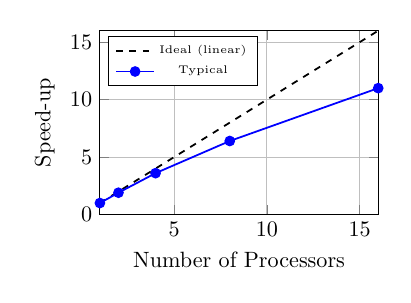
\begin{tikzpicture}[scale=0.8]
                \begin{axis}[
                    width=6cm,
                    height=4.5cm,
                    xlabel={Number of Processors},
                    ylabel={Speed-up},
                    legend pos=north west,
                    grid=major,
                    xmin=1, xmax=16,
                    ymin=0, ymax=16,
                    legend style={font=\tiny}
                ]
                \addplot[black, dashed, thick, domain=1:16] {x};
                \addlegendentry{Ideal (linear)}

                \addplot[blue, thick, mark=*, samples at={1,2,4,8,16}] coordinates {
                    (1,1) (2,1.9) (4,3.6) (8,6.4) (16,11)
                };
                \addlegendentry{Typical}
                \end{axis}
            \end{tikzpicture}
        \end{column}
    \end{columns}
\end{frame}

\begin{frame}{Strong Scaling vs Weak Scaling}
	\footnotesize
    \begin{columns}[T]
        \begin{column}{0.5\textwidth}
            \textbf{Strong Scaling:}
            \begin{itemize}
                \item \textbf{Fixed total problem size}
                \item Increase number of processors
                \item Measure time to solution
            \end{itemize}
            \vskip0.5em
            \textbf{Goal:} Solve the same problem faster
            \vskip0.5em
            \textbf{Example:}
            \begin{itemize}
                \item Problem: Process 1M data points
                \item 1 core: 100 seconds
                \item 2 cores: 55 seconds (each processes 500K)
                \item 4 cores: 30 seconds (each processes 250K)
            \end{itemize}
            \vskip0.5em
            \textbf{Challenge:} Communication overhead increases
        \end{column}
        \begin{column}{0.5\textwidth}
            \textbf{Weak Scaling:}
            \begin{itemize}
                \item \textbf{Fixed problem size per processor}
                \item Increase processors and total problem size together
                \item Measure time per processor
            \end{itemize}
            \vskip0.5em
            \textbf{Goal:} Solve bigger problems in same time
            \vskip0.5em
            \textbf{Example:}
            \begin{itemize}
                \item 1 core: 1M points in 100 seconds
                \item 2 cores: 2M points in 100 seconds
                \item 4 cores: 4M points in 100 seconds
            \end{itemize}
            \vskip0.5em
            \textbf{Challenge:} Memory and communication patterns
        \end{column}
    \end{columns}
    \vskip1em
    \textbf{When to use which:}
    \begin{itemize}
        \item Strong scaling: Fixed problem, want faster results
        \item Weak scaling: Problem scales with resources, want to solve bigger problems
    \end{itemize}
\end{frame}

\begin{frame}{Deriving Amdahl's Law}
	\footnotesize
    \textbf{The Fundamental Question:} What limits parallel speedup?
    \vskip.2em
    \begin{columns}[T]
        \begin{column}{0.5\textwidth}
            \textbf{Key Insight:}
            \begin{itemize}
                \item Every program has serial and parallel parts
                \item Serial part cannot be sped up
                \item Only parallel part benefits from more processors
            \end{itemize}
            \vskip1em
            \textbf{Let's derive:}
            \begin{enumerate}
                \item Let $T$ = total time on 1 processor
                \item Let $p$ = fraction that's parallelizable
                \item Let $(1-p)$ = serial fraction
            \end{enumerate}
        \end{column}
        \begin{column}{0.5\textwidth}
            \textbf{With $N$ processors:}
            \begin{itemize}
                \item Serial time: $(1-p) \times T$
                \item Parallel time: $\frac{p \times T}{N}$
                \item Total time: $(1-p) \times T + \frac{p \times T}{N}$
            \end{itemize}
            \vskip0.5em
            \textbf{Speed-up:}
            \[
            S(N) = \frac{T}{(1-p) \times T + \frac{p \times T}{N}}
            \]
            \vskip0.5em
            Simplify by dividing by $T$:
            \[
            S(N) = \frac{1}{(1-p) + \frac{p}{N}}
            \]
        \end{column}
    \end{columns}
    \vskip.2em
    \textbf{Implication:} Maximum speedup is limited by serial fraction!
\end{frame}

\begin{frame}[fragile]{Amdahl's Law: The Speedup Limit}
	\footnotesize
    \begin{columns}[T]
        \begin{column}{0.5\textwidth}
            \textbf{The Formula:}
            \[
            S(n) = \frac{1}{(1-p) + \frac{p}{n}}
            \]
            where:
            \begin{itemize}
                \item $S(n)$ = speedup with $n$ processors
                \item $p$ = parallel fraction of code
                \item $(1-p)$ = serial fraction
            \end{itemize}
            \vskip1em
            \textbf{Key Insights:}
            \begin{itemize}
                \item Even 5\% serial code limits speedup to 20×
                \item As $n \to \infty$: $S \to \frac{1}{1-p}$
                \item Adding more processors has diminishing returns
            \end{itemize}
        \end{column}
        \begin{column}{0.5\textwidth}
            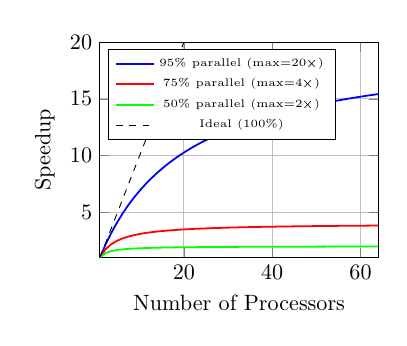
\begin{tikzpicture}[scale=0.8]
                \begin{axis}[
                    width=6cm,
                    height=5cm,
                    xlabel={Number of Processors},
                    ylabel={Speedup},
                    legend pos=north west,
                    grid=major,
                    xmin=1, xmax=64,
                    ymin=1, ymax=20,
                    legend style={font=\tiny}
                ]
                \addplot[blue, thick, domain=1:64, samples=50] {1/((1-0.95) + 0.95/x)};
                \addlegendentry{95\% parallel (max=20×)}

                \addplot[red, thick, domain=1:64, samples=50] {1/((1-0.75) + 0.75/x)};
                \addlegendentry{75\% parallel (max=4×)}

                \addplot[green, thick, domain=1:64, samples=50] {1/((1-0.50) + 0.50/x)};
                \addlegendentry{50\% parallel (max=2×)}

                \addplot[black, dashed, domain=1:20] {x};
                \addlegendentry{Ideal (100\%)}
                \end{axis}
            \end{tikzpicture}
            \vskip0.5em
            \textbf{Lesson:} Optimize serial portions first!
        \end{column}
    \end{columns}
\end{frame}

\begin{frame}[fragile]{Gustafson's Law: Scaling the Problem}
	\vspace{-1em}
	\footnotesize
    \begin{columns}[T]
        \begin{column}{0.5\textwidth}
            \textbf{A Different Perspective:}
            \begin{itemize}
                \item Amdahl assumes \textbf{fixed problem size}
                \item Gustafson assumes \textbf{fixed execution time}
                \item Scale the problem with processors
            \end{itemize}
            \vskip0.5em
            \textbf{The Formula:}
            \[
            S(N) = N - s(N-1) = s + p \cdot N
            \]
            where:
            \begin{itemize}
                \item $s$ = serial fraction
                \item $p$ = parallel fraction ($p = 1-s$)
                \item $N$ = number of processors
            \end{itemize}
            \vskip0.5em
            \textbf{Key Insight:} Speedup grows \textbf{linearly} with $N$!
        \end{column}
        \begin{column}{0.5\textwidth}
            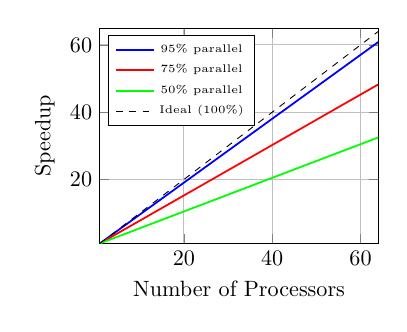
\begin{tikzpicture}[scale=0.8]
                \begin{axis}[
                    width=6cm,
                    height=5cm,
                    xlabel={Number of Processors},
                    ylabel={Speedup},
                    legend pos=north west,
                    grid=major,
                    xmin=1, xmax=64,
                    ymin=1, ymax=65,
                    legend style={font=\tiny}
                ]
                \addplot[blue, thick, domain=1:64, samples=50] {0.05 + 0.95*x};
                \addlegendentry{95\% parallel}

                \addplot[red, thick, domain=1:64, samples=50] {0.25 + 0.75*x};
                \addlegendentry{75\% parallel}

                \addplot[green, thick, domain=1:64, samples=50] {0.50 + 0.50*x};
                \addlegendentry{50\% parallel}

                \addplot[black, dashed, domain=1:64] {x};
                \addlegendentry{Ideal (100\%)}
                \end{axis}
            \end{tikzpicture}
            \vskip0.5em
            \textbf{Lesson:} With larger problems, parallelism pays off!
        \end{column}
    \end{columns}
\end{frame}

\begin{frame}{\LARGE Amdahl vs Gustafson: When to Use Which}
	\vspace{-1em}
	\footnotesize
    \begin{columns}[T]
        \begin{column}{0.5\textwidth}
            \textbf{Amdahl's Law:}
            \begin{itemize}
                \item Fixed problem size
                \item Strong scaling scenario
                \item Pessimistic view
                \item Good for: "How fast can I solve \textit{this} problem?"
            \end{itemize}
            \vskip.2em
            \textbf{Example:}
            \begin{itemize}
                \item Analyze today's dataset faster
                \item Real-time processing constraints
                \item Fixed input size applications
            \end{itemize}
        \end{column}
        \begin{column}{0.5\textwidth}
            \textbf{Gustafson's Law:}
            \begin{itemize}
                \item Scaled problem size
                \item Weak scaling scenario
                \item Optimistic view
                \item Good for: "How big a problem can I solve?"
            \end{itemize}
            \vskip.2em
            \textbf{Example:}
            \begin{itemize}
                \item Higher resolution simulations
                \item Larger training datasets
                \item More parameter combinations
            \end{itemize}
        \end{column}
    \end{columns}
    \vskip1em
    \textbf{Reality:} Most HPC users benefit from Gustafson's perspective---more resources let you tackle bigger, more interesting problems!
\end{frame}

%%%%%%%%%%%%%%%%%%%%%%%%%%%%%%%%%%%%%%%%%%%%%%%%%%%%%%%%%%%%%%%%%%%%%%%%%%
\section{Cluster Workflow and SLURM Basics}
%%%%%%%%%%%%%%%%%%%%%%%%%%%%%%%%%%%%%%%%%%%%%%%%%%%%%%%%%%%%%%%%%%%%%%%%%%

\begin{frame}{What is SLURM?}
	\footnotesize
    \textbf{Simple Linux Utility for Resource Management}
    \vskip1em
    \begin{columns}[T]
        \begin{column}{0.7\textwidth}
            \textbf{Functions:}
            \begin{itemize}
                \item \textbf{Resource Manager}: Allocate compute resources
                \item \textbf{Job Scheduler}: Queue and prioritize jobs
                \item \textbf{Workload Manager}: Monitor job execution
            \end{itemize}
            \vskip1em
            \textbf{Why SLURM?}
            \begin{itemize}
                \item Fair sharing of resources
                \item Prevents conflicts
                \item Optimizes cluster utilization
                \item Provides accounting and reporting
            \end{itemize}
        \end{column}
        \begin{column}{0.3\textwidth}
            \textbf{Job Lifecycle:} \\
            \vspace{2em}
            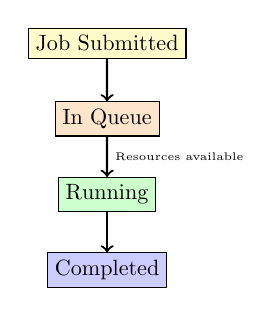
\begin{tikzpicture}[node distance=1.2cm, scale=0.7, every node/.style={scale=0.8}]
                \node[draw, rectangle, fill=yellow!20] (submit) {Job Submitted};
                \node[draw, rectangle, fill=orange!20, below of=submit] (queue) {In Queue};
                \node[draw, rectangle, fill=green!20, below of=queue] (run) {Running};
                \node[draw, rectangle, fill=blue!20, below of=run] (complete) {Completed};

                \draw[->, thick] (submit) -- (queue);
                \draw[->, thick] (queue) -- (run) node[midway, right] {\tiny Resources available};
                \draw[->, thick] (run) -- (complete);
            \end{tikzpicture}
        \end{column}
    \end{columns}
\end{frame}

\begin{frame}{Common SLURM Commands}
	\scriptsize
    \begin{tabular}{p{4.5cm}p{6.5cm}}
        \toprule
        \textbf{Command} & \textbf{Description} \\
        \midrule
        \texttt{sbatch script.sh} & Submit a batch job \\
        \texttt{squeue} & View job queue (all users) \\
        \texttt{squeue -u \$USER} & View your jobs \\
        \texttt{scancel <jobid>} & Cancel a job \\
        \texttt{sinfo} & View cluster node information \\
        \texttt{srun command} & Run command interactively \\
        \texttt{scontrol show job <jobid>} & View detailed job info \\
        \texttt{sacct} & View job accounting information \\
        \texttt{salloc} & Allocate resources for interactive use \\
        \bottomrule
    \end{tabular}
    \vskip0.8em
    \footnotesize
    \textbf{Useful squeue options:}
    \begin{itemize}
        \item \texttt{-l}: Long format with more details
        \item \texttt{--start}: Show estimated start time
        \item \texttt{-t RUNNING}: Filter by job state (PENDING, RUNNING, etc.)
    \end{itemize}
\end{frame}

\begin{frame}[fragile]{Anatomy of a SLURM Job Script}
    \begin{columns}[T]
        \begin{column}{0.5\textwidth}
            \textbf{Basic Structure:}
            \begin{lstlisting}[language=bash, basicstyle=\tiny\ttfamily]
#!/bin/bash
#SBATCH --job-name=myjob
#SBATCH --output=output_%j.txt
#SBATCH --error=error_%j.txt
#SBATCH --time=01:00:00
#SBATCH --nodes=1
#SBATCH --ntasks=1
#SBATCH --cpus-per-task=4
#SBATCH --mem=8G

# Load modules
module load python/3.9

# Set environment
export OMP_NUM_THREADS=4

# Run application
python my_script.py
            \end{lstlisting}
        \end{column}
        \begin{column}{0.5\textwidth}
            \scriptsize
            \textbf{Key Options:}
            \begin{itemize}
                \item \texttt{--job-name}: Job identifier
                \item \texttt{--output/--error}: Log files
                \item \texttt{--time}: Max runtime (HH:MM:SS)
                \item \texttt{--nodes}: Number of nodes
                \item \texttt{--ntasks}: Number of tasks
                \item \texttt{--cpus-per-task}: Cores per task
                \item \texttt{--mem}: Memory per node
                \item \texttt{--mem-per-cpu}: Memory per core
            \end{itemize}
            \vskip0.5em
            \textbf{Special Variables:}
            \begin{itemize}
                \item \texttt{\%j}: Job ID
                \item \texttt{\%x}: Job name
                \item \texttt{\%N}: Node name
            \end{itemize}
        \end{column}
    \end{columns}
\end{frame}

\begin{frame}[fragile]{Example: Serial Job}
    \footnotesize
    \textbf{Simplest case: Single core job}
    \vskip0.4em
    \begin{lstlisting}[language=bash, basicstyle=\scriptsize\ttfamily]
#!/bin/bash
#SBATCH --job-name=serial_job
#SBATCH --output=serial_%j.log
#SBATCH --ntasks=1
#SBATCH --cpus-per-task=1
#SBATCH --mem=2G
#SBATCH --time=00:30:00

echo "Running on host: $(hostname)"
echo "Job ID: $SLURM_JOB_ID"
echo "Number of cores: $SLURM_CPUS_PER_TASK"

python my_serial_script.py
    \end{lstlisting}
    \vskip0.4em
    \textbf{Resources:} 1 node, 1 core, 2 GB RAM, 30 minutes
\end{frame}

\begin{frame}[fragile]{Example: Multi-threaded {\LARGE (OpenMP)} Job}
    \footnotesize
    \textbf{Using multiple cores on a single node}
    \vskip0.2em
    \begin{lstlisting}[language=bash, basicstyle=\tiny\ttfamily]
#!/bin/bash
#SBATCH --job-name=openmp_job
#SBATCH --output=openmp_%j.log
#SBATCH --ntasks=1
#SBATCH --cpus-per-task=16
#SBATCH --mem=32G
#SBATCH --time=02:00:00

module load gcc/11.2.0

export OMP_NUM_THREADS=$SLURM_CPUS_PER_TASK
echo "Using $OMP_NUM_THREADS OpenMP threads"

./my_openmp_program
    \end{lstlisting}
    \vskip0.2em
    \textbf{Resources:} 1 task, 16 cores for threading, 32 GB RAM
\end{frame}

\begin{frame}[fragile]{Example: MPI Job (Distributed)}
    \footnotesize
    \textbf{Multiple tasks across nodes}
    \vskip0.8em
    \begin{lstlisting}[language=bash, basicstyle=\tiny\ttfamily]
#!/bin/bash
#SBATCH --job-name=mpi_job
#SBATCH --output=mpi_%j.log
#SBATCH --nodes=4
#SBATCH --ntasks=64
#SBATCH --cpus-per-task=1
#SBATCH --mem-per-cpu=2G
#SBATCH --time=04:00:00

module load openmpi/4.1.1

echo "Running on $SLURM_NNODES nodes"
echo "Total tasks: $SLURM_NTASKS"

mpirun ./my_mpi_program
    \end{lstlisting}
    \vskip0.8em
    \textbf{Resources:} 4 nodes, 64 MPI tasks (16 per node), 128 GB total RAM
\end{frame}

\begin{frame}[fragile]{Example: Hybrid MPI + OpenMP Job}
    \footnotesize
    \textbf{Combining distributed and shared memory parallelism}
    \vskip0.8em
    \begin{lstlisting}[language=bash, basicstyle=\tiny\ttfamily]
#!/bin/bash
#SBATCH --job-name=hybrid_job
#SBATCH --output=hybrid_%j.log
#SBATCH --nodes=4
#SBATCH --ntasks=16
#SBATCH --cpus-per-task=8
#SBATCH --mem=256G
#SBATCH --time=06:00:00

module load gcc/11.2.0 openmpi/4.1.1

export OMP_NUM_THREADS=$SLURM_CPUS_PER_TASK
echo "MPI tasks: $SLURM_NTASKS"
echo "OpenMP threads per task: $OMP_NUM_THREADS"

mpirun ./my_hybrid_program
    \end{lstlisting}
    \vskip0.8em
    \textbf{Resources:} 4 nodes, 16 MPI tasks (4 per node), 8 threads per task = 128 cores
\end{frame}


\begin{frame}{Resource Allocation Strategies}
	\footnotesize
    \textbf{Choosing the Right Configuration}
    \vskip1em
    \tiny
    \begin{tabular}{p{3.5cm}p{3cm}p{4.5cm}}
        \toprule
        \textbf{Job Type} & \textbf{SLURM Config} & \textbf{Use Case} \\
        \midrule
        \textbf{Serial Job} & 
        \texttt{--ntasks=1} \newline \texttt{--cpus-per-task=1} & 
        Single-threaded code, simple scripts, many independent runs \\
        \midrule
        \textbf{Multi-threaded} & 
        \texttt{--ntasks=1} \newline \texttt{--cpus-per-task=N} & 
        OpenMP/threads, shared memory code, single node sufficient \\
        \midrule
        \textbf{MPI} & 
        \texttt{--ntasks=N} \newline \texttt{--cpus-per-task=1} & 
        Distributed memory, large scale problems, multiple nodes needed \\
        \midrule
        \textbf{Hybrid} \newline \textbf{(MPI+OpenMP)} & 
        \texttt{--ntasks=M} \newline \texttt{--cpus-per-task=N} & 
        Very large problems, reduced MPI overhead, maximum scalability \\
        \bottomrule
    \end{tabular}
    \vskip1em
    \textbf{Decision Guide:}
    \begin{itemize}
        \item Serial: Code not parallelizable or testing phase
        \item Multi-threaded: Code supports threading, problem fits on one node
        \item MPI: Need multiple nodes, problem naturally decomposes
        \item Hybrid: Maximize efficiency on large-scale runs
    \end{itemize}
\end{frame}

\begin{frame}[fragile]{Job Arrays: Running Many Similar Jobs}
	\footnotesize
    \textbf{Scenario:} Need to run same program with different parameters
    \vskip.2em
    \textbf{Without Job Arrays:} Submit 100 separate jobs, manage 100 job IDs (tedious!)
    \vskip0.1em
    \textbf{With Job Arrays:} Single submission, one job ID with array indices (easy!)
    \vskip.2em
    \begin{lstlisting}[language=bash, basicstyle=\tiny\ttfamily]
#!/bin/bash
#SBATCH --job-name=array_job
#SBATCH --output=job_%A_%a.log
#SBATCH --array=1-100
#SBATCH --ntasks=1
#SBATCH --cpus-per-task=1
#SBATCH --mem=2G
#SBATCH --time=01:00:00

# SLURM_ARRAY_TASK_ID contains the current array index (1-100)
PARAM=$SLURM_ARRAY_TASK_ID
echo "Processing parameter: $PARAM"
python process.py --id $PARAM
    \end{lstlisting}
\end{frame}

\begin{frame}{Job Arrays: Advanced Features}
    \begin{columns}[T]
	\begin{column}{0.5\textwidth}
	\footnotesize
    \textbf{Array Syntax Options:}
    \begin{itemize}
        \item \texttt{--array=1-100}: Indices 1 through 100
        \item \texttt{--array=1-100:10}: Every 10th index (1, 11, 21, ...)
        \item \texttt{--array=1,5,10,15}: Specific indices
        \item \texttt{--array=1-100\%10}: Limit to 10 concurrent tasks
    \end{itemize}
    \vskip.2em
    \textbf{Special Variables:}
    \begin{itemize}
	\item \texttt{\%A}: Job array master ID
	\item \texttt{\%a}: Individual array task ID
	\item \texttt{\$SLURM\_ARRAY\_TASK\_ID}: Current array index
	\end{itemize}
    \vskip.2em
    \end{column}
	\begin{column}{0.5\textwidth}
	\footnotesize
	\vspace{5em}
    \textbf{Benefits:}
    \begin{itemize}
        \item Easier management (one job ID)
        \item Automatic resource scheduling
        \item Better for cluster scheduler
        \item Can limit concurrent tasks
    \end{itemize}
    \end{column}
    \end{columns}
\end{frame}

\begin{frame}[fragile]{Interactive Jobs with srun}
    \footnotesize
    \textbf{Run a single command interactively:}
    \vskip0.8em
    \begin{lstlisting}[language=bash, basicstyle=\scriptsize\ttfamily]
# Interactive single command
srun --ntasks=1 \
     --cpus-per-task=4 \
     --mem=8G \
     --time=01:00:00 \
     python my_script.py
    \end{lstlisting}
    \vskip1em
    \textbf{Characteristics:}
    \begin{itemize}
        \item Blocks until complete
        \item Output to terminal
        \item Good for testing and debugging
        \item Waits for resources if not immediately available
    \end{itemize}
\end{frame}

\begin{frame}[fragile]{Interactive Jobs with salloc}
    \footnotesize
    \textbf{Allocate resources for interactive shell:}
    \vskip0.2em
    \begin{lstlisting}[language=bash, basicstyle=\tiny\ttfamily]
# Allocate resources
salloc --nodes=1 \
       --ntasks=4 \
       --mem=16G \
       --time=02:00:00

# Now on compute node, run multiple commands
hostname
module load python
python  # Interactive Python session
# ... work interactively ...
exit  # Release resources when done
    \end{lstlisting}
    \vskip.1em
    \textbf{Characteristics:}
    \begin{itemize}
        \item Interactive shell session on compute node
        \item Run multiple commands
        \item Good for development and debugging
        \item \textbf{Warning:} Consumes resources even when idle. Use for active work only!
    \end{itemize}
\end{frame}

%%%%%%%%%%%%%%%%%%%%%%%%%%%%%%%%%%%%%%%%%%%%%%%%%%%%%%%%%%%%%%%%%%%%%%%%%%
\section{Translating Concepts into Projects}
%%%%%%%%%%%%%%%%%%%%%%%%%%%%%%%%%%%%%%%%%%%%%%%%%%%%%%%%%%%%%%%%%%%%%%%%%%

\begin{frame}{{\Large Programming Languages and Parallel Computing}}
    \footnotesize
    \begin{tabular}{p{2cm}p{4cm}p{6cm}}
        \toprule
        \textbf{Language} & \textbf{Paradigm} & \textbf{Common Tools} \\
        \midrule
        Python & Multi-threading & \texttt{threading}, \texttt{multiprocessing}, \texttt{joblib} \\
               & Message passing & \texttt{mpi4py} \\
               & Vectorization & \texttt{numpy}, \texttt{numba} \\
        \midrule
        Julia & Multi-threading & \texttt{Threads.@threads}, \texttt{@spawn} \\
              & Message passing & \texttt{MPI.jl} \\
              & Distributed & \texttt{Distributed.jl}, \texttt{@distributed} \\
        \midrule
        R & Multi-threading & \texttt{parallel}, \texttt{foreach} \\
          & Message passing & \texttt{Rmpi}, \texttt{pbdMPI} \\
          & Vectorization & Built-in vectorized operations \\
        \midrule
        C/C++ & Multi-threading & OpenMP, pthreads, TBB \\
              & Message passing & MPI \\
              & Vectorization & Compiler auto-vectorization \\
        %\bottomrule
    \end{tabular}
\end{frame}

\begin{frame}[fragile]{{\LARGE Python: Multi-threading vs Multiprocessing}}
	\vspace{-1em}
    \footnotesize
    \begin{columns}[T]
        \begin{column}{0.5\textwidth}
            \textbf{Threading (GIL limitation):}
            \begin{lstlisting}[language=Python, basicstyle=\tiny\ttfamily]
from concurrent.futures import ThreadPoolExecutor
import numpy as np

def compute(x):
    # Good for I/O-bound tasks
    return np.sqrt(x)

with ThreadPoolExecutor(max_workers=4) as ex:
    results = ex.map(compute, range(100))
            \end{lstlisting}
            \vskip0.2em
            \textbf{Multiprocessing:}
            \begin{lstlisting}[language=Python, basicstyle=\tiny\ttfamily]
from multiprocessing import Pool

def compute(x):
    # Good for CPU-bound tasks
    return x ** 2

with Pool(processes=4) as pool:
    results = pool.map(compute, range(100))
            \end{lstlisting}
        \end{column}
        \begin{column}{0.5\textwidth}
            \textbf{Key Differences:}
            \begin{itemize}
                \item \textbf{Threading:} Shared memory, GIL-limited
                \item \textbf{Multiprocessing:} Separate processes, true parallelism
            \end{itemize}
            \vskip1em
            \textbf{SLURM Configuration:}
            \begin{lstlisting}[language=bash, basicstyle=\tiny\ttfamily]
# For multiprocessing
#SBATCH --ntasks=1
#SBATCH --cpus-per-task=4

# In Python script
import os
from multiprocessing import cpu_count
n_cores = int(os.getenv(
    'SLURM_CPUS_PER_TASK', 
    cpu_count()))
            \end{lstlisting}
        \end{column}
    \end{columns}
\end{frame}

\begin{frame}[fragile]{Python: MPI with mpi4py}
	\vspace{-1em}
    \footnotesize
    \textbf{Distributed memory parallelism in Python}
    \vskip0.2em
    \begin{columns}[T]
        \begin{column}{0.5\textwidth}
            \textbf{Example Code:}
            \begin{lstlisting}[language=Python, basicstyle=\tiny\ttfamily]
from mpi4py import MPI
import numpy as np

comm = MPI.COMM_WORLD
rank = comm.Get_rank()
size = comm.Get_size()

# Each process computes part
n_local = 1000
data = np.random.rand(n_local)
local_sum = np.sum(data)

# Reduce to get total sum
total_sum = comm.reduce(
    local_sum, 
    op=MPI.SUM, 
    root=0)

if rank == 0:
    print(f"Total: {total_sum}")
            \end{lstlisting}
        \end{column}
        \begin{column}{0.5\textwidth}
            \textbf{SLURM Job Script:}
            \begin{lstlisting}[language=bash, basicstyle=\tiny\ttfamily]
#!/bin/bash
#SBATCH --ntasks=16
#SBATCH --cpus-per-task=1
#SBATCH --mem-per-cpu=2G
#SBATCH --time=01:00:00

module load openmpi python/3.9

mpirun python my_mpi_script.py
            \end{lstlisting}
            \vskip0.2em
            \textbf{Key Points:}
            \begin{itemize}
                \item Use \texttt{mpirun} to launch
                \item Each process has unique rank
                \item Communication via MPI functions
                \item Scales across multiple nodes
            \end{itemize}
        \end{column}
    \end{columns}
\end{frame}

\begin{frame}[fragile]{Julia: Multi-threading}
    \small
    \begin{columns}[T]
        \begin{column}{0.5\textwidth}
            \textbf{Multi-threading Example:}
            \begin{lstlisting}[language=Python, basicstyle=\tiny\ttfamily]
using Base.Threads

# Set threads with environment variable
# export JULIA_NUM_THREADS=4

function parallel_sum(arr)
    result = zeros(nthreads())
    @threads for i in eachindex(arr)
        tid = threadid()
        result[tid] += arr[i]
    end
    return sum(result)
end

# Test
arr = rand(1000000)
total = parallel_sum(arr)
            \end{lstlisting}
        \end{column}
        \begin{column}{0.5\textwidth}
            \textbf{SLURM Configuration:}
            \begin{lstlisting}[language=bash, basicstyle=\tiny\ttfamily]
#!/bin/bash
#SBATCH --ntasks=1
#SBATCH --cpus-per-task=8
#SBATCH --mem=16G
#SBATCH --time=02:00:00

module load julia/1.8

# For threading
export JULIA_NUM_THREADS=$SLURM_CPUS_PER_TASK

julia my_script.jl
            \end{lstlisting}
            \vskip0.8em
            \textbf{Features:}
            \begin{itemize}
                \item Native threading support
                \item Easy to use with \texttt{@threads}
                \item Good performance
                \item Set thread count via environment
            \end{itemize}
        \end{column}
    \end{columns}
\end{frame}

\begin{frame}[fragile]{Julia: Distributed Computing}
    \small
    \begin{columns}[T]
        \begin{column}{0.5\textwidth}
            \textbf{Distributed.jl:}
            \begin{lstlisting}[language=Python, basicstyle=\tiny\ttfamily]
using Distributed

# Add 4 worker processes
addprocs(4)

# Function available on all workers
@everywhere function compute(x)
    return x^2
end

# Parallel reduction
results = @distributed (+) for i = 1:100
    compute(i)
end

println("Sum of squares: $results")
            \end{lstlisting}
        \end{column}
        \begin{column}{0.5\textwidth}
            \textbf{MPI.jl:}
            \begin{lstlisting}[language=Python, basicstyle=\tiny\ttfamily]
using MPI

MPI.Init()
comm = MPI.COMM_WORLD
rank = MPI.Comm_rank(comm)
size = MPI.Comm_size(comm)

# Each rank does work
local_result = rank * 10

# Gather results
all_results = MPI.Gather(
    local_result, 0, comm)

if rank == 0
    println("Results: $all_results")
end
            \end{lstlisting}
        \end{column}
    \end{columns}
    \vskip0.8em
    \textbf{Choice:} Use Distributed.jl for within-cluster, MPI.jl for large-scale HPC
\end{frame}

\begin{frame}[fragile]{R: Parallel Package - Part 1}
    \small
    \begin{columns}[T]
        \begin{column}{0.5\textwidth}
            \textbf{Using foreach:}
            \begin{lstlisting}[language=Python, basicstyle=\tiny\ttfamily]
library(foreach)
library(doParallel)

# Register parallel backend
cl <- makeCluster(4)
registerDoParallel(cl)

# Parallel loop
results <- foreach(
    i=1:100, 
    .combine=c) %dopar% {
    # Computation
    i^2
}

stopCluster(cl)
            \end{lstlisting}
        \end{column}
        \begin{column}{0.5\textwidth}
            \textbf{Using mclapply:}
            \begin{lstlisting}[language=Python, basicstyle=\tiny\ttfamily]
library(parallel)

# Detect cores
ncores <- detectCores()

# Parallel apply
results <- mclapply(
    1:100, 
    function(x) x^2,
    mc.cores = ncores)

# Convert to vector
results <- unlist(results)
            \end{lstlisting}
        \end{column}
    \end{columns}
    \vskip1em
    \textbf{Note:} \texttt{mclapply} uses forking (Unix only), \texttt{foreach} works cross-platform
\end{frame}

\begin{frame}[fragile]{R: Parallel Package - Part 2}
    \footnotesize
    \begin{columns}[T]
        \begin{column}{0.5\textwidth}
            \textbf{SLURM Job Script:}
            \begin{lstlisting}[language=bash, basicstyle=\tiny\ttfamily]
#!/bin/bash
#SBATCH --ntasks=1
#SBATCH --cpus-per-task=8
#SBATCH --mem=16G
#SBATCH --time=01:00:00

module load r/4.2

# Set cores from SLURM
export R_NCORES=$SLURM_CPUS_PER_TASK

Rscript my_script.R
            \end{lstlisting}
        \end{column}
        \begin{column}{0.5\textwidth}
            \textbf{In R script:}
            \begin{lstlisting}[language=Python, basicstyle=\tiny\ttfamily]
# Get cores from environment
ncores <- as.integer(
    Sys.getenv("R_NCORES", "1"))

# Use with foreach
cl <- makeCluster(ncores)
registerDoParallel(cl)

# ... rest of code ...

stopCluster(cl)
            \end{lstlisting}
        \end{column}
    \end{columns}
    \vskip1em
    \textbf{Best Practices:}
    \begin{itemize}
        \item Always read core count from SLURM environment
        \item Remember to stop clusters when done
        \item Use \texttt{.combine} to control result aggregation
    \end{itemize}
\end{frame}

\begin{frame}{Debugging Parallel Programs}
	\vspace{-1em}
    \footnotesize
    \begin{columns}[T]
        \begin{column}{0.5\textwidth}
            \textbf{Common Issues:}
            \begin{itemize}
                \item Race conditions
                \item Deadlocks
                \item Memory errors
                \item Load imbalance
                \item Communication bottlenecks
            \end{itemize}
            \vskip0.8em
            \textbf{Debugging Strategies:}
            \begin{itemize}
                \item Start with serial version
                \item Test with small problem size
                \item Use print statements
                \item Check with debuggers (GDB, DDT)
                \item Profile code performance
            \end{itemize}
        \end{column}
        \begin{column}{0.5\textwidth}
            \textbf{Best Practices:}
            \begin{enumerate}
                \item \textbf{Validate serial code first}
                \item \textbf{Start with small scale}
                \begin{itemize}
                    \tiny
                    \item 2-4 processes/threads
                    \item Small data sets
                \end{itemize}
                \item \textbf{Compare results}
                \begin{itemize}
                    \tiny
                    \item Serial vs parallel
                    \item Different core counts
                \end{itemize}
                \item \textbf{Use debugging tools}
                \begin{itemize}
                    \tiny
                    \item Valgrind for memory
                    \item GDB for segfaults
                    \item Profilers for performance
                \end{itemize}
                \item \textbf{Monitor resource usage}
                \begin{itemize}
                    \tiny
                    \item Check CPU utilization
                    \item Memory consumption
                    \item Network traffic (MPI)
                \end{itemize}
            \end{enumerate}
        \end{column}
    \end{columns}
\end{frame}

\begin{frame}{Performance Optimization Tips}
	\vspace{-1em}
    \footnotesize
    \begin{columns}[T]
        \begin{column}{0.5\textwidth}
            \begin{enumerate}
                \item \textbf{Profile Before Optimizing}
                \begin{itemize}
                    \item Identify bottlenecks
                    \item Focus on hot spots
                    \item Measure, don't guess
                \end{itemize}

                \item \textbf{Optimize Serial Code First}
                \begin{itemize}
                    \item Algorithm improvements
                    \item Data structures
                    \item Memory access patterns
                \end{itemize}

                \item \textbf{Minimize Communication}
                \begin{itemize}
                    \item Reduce MPI calls
                    \item Batch communications
                    \item Overlap compute and comm.
                \end{itemize}
            \end{enumerate}
        \end{column}
        \begin{column}{0.5\textwidth}
            \begin{enumerate}
                \setcounter{enumi}{3}
                \item \textbf{Balance Load}
                \begin{itemize}
                    \item Equal work distribution
                    \item Dynamic load balancing
                    \item Avoid idle processes
                \end{itemize}

                \item \textbf{Use Appropriate Tools}
                \begin{itemize}
                    \item Vectorized operations
                    \item Efficient libraries (BLAS, LAPACK)
                    \item Compiler optimizations
                \end{itemize}

                \item \textbf{Memory Efficiency}
                \begin{itemize}
                    \item Cache-friendly access
                    \item Minimize allocations
                    \item Avoid memory leaks
                \end{itemize}
            \end{enumerate}
        \end{column}
    \end{columns}
\end{frame}

\begin{frame}[fragile]{Scaling Studies}
    \footnotesize
    \begin{columns}[T]
        \begin{column}{0.5\textwidth}
            \textbf{Strong Scaling:}
            \begin{itemize}
                \item Fixed problem size
                \item Increase processors
                \item Measure time to solution
                \item Goal: Linear speedup
            \end{itemize}
            \vskip0.5em
            \textbf{Weak Scaling:}
            \begin{itemize}
                \item Fixed problem per processor
                \item Increase processors and problem
                \item Measure time per processor
                \item Goal: Constant time
            \end{itemize}

        \end{column}
        \begin{column}{0.5\textwidth}
            \centering
            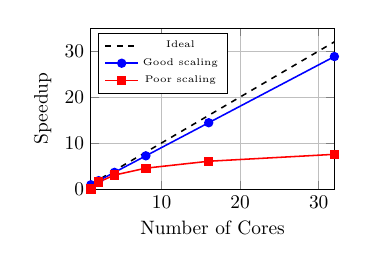
\begin{tikzpicture}[scale=0.7]
                \begin{axis}[
                    width=6cm,
                    height=4.5cm,
                    xlabel={Number of Cores},
                    ylabel={Speedup},
                    legend pos=north west,
                    grid=major,
                    xmin=1, xmax=32,
                    ymin=0, ymax=35,
                    legend style={font=\tiny}
                ]
                \addplot[black, dashed, thick, domain=1:32] {x};
                \addlegendentry{Ideal}

                \addplot[blue, thick, mark=*, samples at={1,2,4,8,16,32}] {x*0.9};
                \addlegendentry{Good scaling}

                \addplot[red, thick, mark=square*, samples at={1,2,4,8,16,32}] {5*log2(x)/log2(10)};
                \addlegendentry{Poor scaling}
                \end{axis}
            \end{tikzpicture}
            \vskip0.5em
            \tiny
            \textbf{What to report:}
            \begin{itemize}
                \item Speedup vs core count
                \item Parallel efficiency
                \item Time breakdown (compute vs comm.)
            \end{itemize}
            \vskip0.5em
			\textbf{Key Metrics:}
			\begin{itemize}
				\item Efficiency = Speedup / N\_cores
				\item Aim for $>$80\% efficiency
			\end{itemize}
        \end{column}
    \end{columns}
\end{frame}

%%%%%%%%%%%%%%%%%%%%%%%%%%%%%%%%%%%%%%%%%%%%%%%%%%%%%%%%%%%%%%%%%%%%%%%%%%
\section{Q\&A and Interaction}
%%%%%%%%%%%%%%%%%%%%%%%%%%%%%%%%%%%%%%%%%%%%%%%%%%%%%%%%%%%%%%%%%%%%%%%%%%

\begin{frame}{{\LARGE Exercise 1: Writing Your First SLURM Script}}
	\vspace{-1em}
    \footnotesize
    \textbf{Task:} Create a simple SLURM job script
    \vskip0.8em
    \begin{enumerate}
        \item Create a script that:
        \begin{itemize}
            \footnotesize
            \item Prints the hostname
            \item Prints available environment variables
            \item Runs a simple calculation
        \end{itemize}
        \item Allocate: 1 node, 4 cores, 8GB RAM, 30 minutes
        \item Submit with \texttt{sbatch}
        \item Check status with \texttt{squeue}
        \item View output logs
    \end{enumerate}
    \vskip0.8em
    \textbf{Bonus:} Modify to use different core counts and compare timing
\end{frame}

\begin{frame}{Exercise 2: Parallel Python Script}
	\vspace{-1em}
    \footnotesize
    \textbf{Task:} Write a parallel Python program
    \vskip0.8em
    \begin{enumerate}
        \item Create a script that:
        \begin{itemize}
		    \footnotesize
            \item Computes sum of squares: $\sum_{i=1}^{N} i^2$
            \item Uses multiprocessing with 4 workers
            \item Compares with serial version
        \end{itemize}
        \item Measure execution time
        \item Create SLURM script to run it
        \item Experiment with different worker counts
    \end{enumerate}
    \vskip0.8em
    \textbf{Questions to explore:}
    \begin{itemize}
        \item How does speedup change with core count?
        \item What's the overhead of parallelization?
    \end{itemize}
\end{frame}

\begin{frame}{Exercise 3: Job Arrays}
	\vspace{-1em}
    \footnotesize
    \textbf{Task:} Use job arrays for parameter sweep
    \vskip0.8em
    \begin{enumerate}
        \item Create a script that takes a parameter as input
        \item Run the same script with parameters 1-20
        \item Use SLURM job arrays
        \item Collect and analyze results
    \end{enumerate}
    \vskip0.8em
    \textbf{Example scenario:}
    \begin{itemize}
        \item Simulate with different random seeds
        \item Process different input files
        \item Test different hyperparameters
    \end{itemize}
    \vskip0.8em
    \textbf{Questions:}
    \begin{itemize}
        \item How to aggregate results from array jobs?
        \item What if some jobs fail?
    \end{itemize}
\end{frame}

\begin{frame}{Common Pitfalls - Resource Issues}
	\vspace{-1em}
    \footnotesize
    \textbf{Resource-Related Problems:}
    \vskip0.8em
    \tiny
    \begin{tabular}{p{4.5cm}p{6cm}}
        \toprule
        \textbf{Pitfall} & \textbf{Solution} \\
        \midrule
        Job stuck in queue & Check node availability with \texttt{sinfo}; reduce resource requests; check time limits \\
        \midrule
        Out of memory (OOM) & Monitor with \texttt{sacct}; increase \texttt{--mem} or \texttt{--mem-per-cpu}; check for memory leaks \\
        \midrule
        Job timeout & Increase \texttt{--time} limit; optimize code; use checkpointing for long jobs \\
        \midrule
        Node allocation issues & Check partition limits; verify account permissions; use \texttt{scontrol show partition} \\
        \bottomrule
    \end{tabular}
    \vskip1em
    \footnotesize
    \textbf{Prevention:}
    \begin{itemize}
        \item Start with test runs on small data
        \item Monitor resource usage with \texttt{sstat} during runs
        \item Use \texttt{sacct} to check completed jobs
    \end{itemize}
\end{frame}

\begin{frame}{{\LARGE Common Pitfalls - Code and Environment}}
	\vspace{-1em}
    \footnotesize
    \textbf{Code and Environment Issues:}
    \vskip0.8em
    \tiny
    \begin{tabular}{p{4.5cm}p{6cm}}
        \toprule
        \textbf{Pitfall} & \textbf{Solution} \\
        \midrule
        Wrong module loaded & Use \texttt{module avail} to find modules; \texttt{module load} correct version; check dependencies \\
        \midrule
        Poor parallel performance & Profile code; check CPU utilization; verify thread/process count; look for load imbalance \\
        \midrule
        Can't find output files & Check working directory; use absolute paths; verify \texttt{\$SLURM\_SUBMIT\_DIR} \\
        \midrule
        Permission denied & Check file permissions; verify group membership; use correct scratch directory \\
        \bottomrule
    \end{tabular}
    \vskip1em
    \footnotesize
    \textbf{Best Practice:}
    \begin{itemize}
        \item Test scripts locally before submitting
        \item Use \texttt{echo} statements to debug paths
    \end{itemize}
\end{frame}

\begin{frame}{Common Pitfalls - Debugging Strategies}
	\vspace{-1em}
    \footnotesize
    \begin{columns}[T]
	    \begin{column}{0.5\textwidth}
		    \textbf{General Debugging Approach:}
		    \vskip.2em
		    \begin{enumerate}
		        \item \textbf{Check Error Logs}
		        \begin{itemize}
				    \footnotesize
		            \item Always read \texttt{stderr} file first
		            \item Look for error messages and stack traces
		            \item Check SLURM output for resource issues
		        \end{itemize}
		        \vskip0.5em

		        \item \textbf{Test Interactively}
		        \begin{itemize}
				    \footnotesize
		            \item Use \texttt{salloc} or \texttt{srun} for interactive sessions
		            \item Run commands manually to isolate issues
		            \item Verify modules and environment variables
		        \end{itemize}
		    \end{enumerate}
		\end{column}
	    \begin{column}{0.5\textwidth}
	        \begin{enumerate}
		        \setcounter{enumi}{2}
		        \item \textbf{Start Small, Scale Up}
		        \begin{itemize}
				    \footnotesize
		            \item Test with minimal resources (1 core, small data)
		            \item Verify correctness before scaling
		            \item Gradually increase resources and problem size
		        \end{itemize}
		        \vskip0.5em

		        \item \textbf{Use Cluster Documentation}
		        \begin{itemize}
				    \footnotesize
		            \item Check cluster-specific quirks
		            \item Review example job scripts
		            \item Contact support if stuck
		        \end{itemize}
	        \end{enumerate}
	    \end{column}
    \end{columns}
\end{frame}

\begin{frame}{Resource Estimation Guidelines}
	\vspace{-1em}
    \footnotesize
    \begin{columns}[T]
	\begin{column}{0.55\textwidth}
    \textbf{How to estimate resources needed:}
    \vskip0.8em
    \begin{enumerate}
        \item \textbf{Memory:}
        \begin{itemize}
    \footnotesize
            \item Run small test with \texttt{/usr/bin/time -v}
            \item Check "Maximum resident set size"
            \item Add 20-30\% buffer
            \item Formula: $\text{mem} = \text{data\_size} \times \text{copies} \times 1.3$
        \end{itemize}
        \vskip0.2em

        \item \textbf{Time:}
        \begin{itemize}
    \footnotesize
            \item Time small problem
            \item Extrapolate to full size
            \item Add buffer for overhead
            \item Consider: $T_{\text{parallel}} \approx \frac{T_{\text{serial}}}{N_{\text{cores}} \times \text{efficiency}}$
        \end{itemize}
        \vskip0.2em
    \end{enumerate}
    \end{column}
	\begin{column}{0.45\textwidth}
	\vspace{6em}
    \begin{enumerate}
	        \setcounter{enumi}{2}
        \item \textbf{Cores:}
        \begin{itemize}
    \footnotesize
            \item Start with small counts (4-8)
            \item Measure speedup
            \item Check parallel efficiency
            \item Don't over-allocate (diminishing returns)
        \end{itemize}
    \end{enumerate}
    \end{column}
    \end{columns}
\end{frame}

\begin{frame}{Best Practices - Job Management}
	\vspace{-1em}
    \footnotesize
    \begin{columns}[T]
        \begin{column}{0.5\textwidth}
            \textbf{Job Submission:}
            \begin{itemize}
			    \footnotesize
                \item Use descriptive job names
                \item Always specify time limits
                \item Use \texttt{\%j} in output files
                \item Test on small scale first
                \item Check queue before submitting many jobs
            \end{itemize}
            \vskip1em
            \textbf{Resource Usage:}
            \begin{itemize}
			    \footnotesize
                \item Request what you need
                \item Don't monopolize resources
                \item Use job arrays for similar jobs
                \item Clean up old files regularly
                \item Monitor your usage
            \end{itemize}
        \end{column}
        \begin{column}{0.5\textwidth}
            \textbf{Job Monitoring:}
            \begin{itemize}
			    \footnotesize
                \item Check job status: \texttt{squeue -u \$USER}
                \item Review completed jobs: \texttt{sacct}, \texttt{seff}
                \item Monitor running jobs: \texttt{sstat}, \texttt{Seffi}
                \item Check efficiency after completion
            \end{itemize}
            \vskip1em
            \textbf{Error Handling:}
            \begin{itemize}
			    \footnotesize
                \item Always capture stderr
                \item Use unique log file names
                \item Implement checkpointing for long jobs
                \item Handle job failures gracefully
            \end{itemize}
        \end{column}
    \end{columns}
\end{frame}

\begin{frame}{Best Practices - Code Development}
	\vspace{-1em}
	\footnotesize
    \begin{columns}[T]
        \begin{column}{0.5\textwidth}
            \textbf{Development Workflow:}
            \begin{itemize}
                \item Version control (git)
                \item Validate serial code first
                \item Test parallel code at small scale
                \item Profile before optimizing
                \item Document your workflow
            \end{itemize}
            \vskip.2em
            \textbf{Testing Strategy:}
            \begin{itemize}
                \item Unit tests for components
                \item Integration tests for workflow
                \item Scaling tests before production
                \item Compare results across scales
                \item Save test datasets
            \end{itemize}
        \end{column}
        \begin{column}{0.5\textwidth}
            \textbf{Code Organization:}
            \begin{itemize}
                \item Separate input/output/code
                \item Use configuration files
                \item Modular design
                \item Clear commenting
                \item README with instructions
            \end{itemize}
            \vskip.2em
            \textbf{Performance:}
            \begin{itemize}
                \item Optimize algorithms first
                \item Use efficient libraries
                \item Minimize I/O operations
                \item Cache frequently-used data
                \item Profile to find bottlenecks
            \end{itemize}
        \end{column}
    \end{columns}
\end{frame}

\begin{frame}{Best Practices - Data Management}
	\vspace{-1em}
    \footnotesize
    \begin{columns}[T]
        \begin{column}{0.5\textwidth}
            \textbf{Storage Strategy:}
            \begin{itemize}
			    \footnotesize
                \item \textbf{Use work/scratch} for temporary files
                \item \textbf{Back up} important results to the NAS
                \item Compress large files
                \item \textbf{Clean up} after jobs complete
                \item Document data provenance
            \end{itemize}
            \vskip1em
            \textbf{File Organization:}
            \begin{itemize}
			    \footnotesize
                \item Meaningful directory structure
                \item Consistent naming conventions
                \item Separate raw and processed data
                \item Use metadata files
            \end{itemize}
        \end{column}
        \begin{column}{0.5\textwidth}
            \textbf{I/O Optimization:}
            \begin{itemize}
			    \footnotesize
                \item Batch small files
                \item Use appropriate formats (HDF5, NetCDF)
                \item Minimize random access
                \item Consider parallel I/O for large data
                \item Profile I/O performance
            \end{itemize}
            \vskip1em
            \textbf{Collaboration:}
            \begin{itemize}
			    \footnotesize
                \item \textbf{Communicate} with the team
                \item \textbf{Share} code via repositories
                \item \textbf{Document} dependencies
                \item \textbf{Use containers} if available
                \item Follow cluster policies
            \end{itemize}
        \end{column}
    \end{columns}
\end{frame}

\begin{frame}{Additional Resources}
	\vspace{-1em}
    \footnotesize
    \textbf{Documentation:}
    \begin{itemize}
        \footnotesize
        \item SLURM Official Documentation: \texttt{https://slurm.schedmd.com/}
        \item Your cluster's wiki/documentation
        \item \texttt{man sbatch}, \texttt{man srun}, etc.
    \end{itemize}
    \vskip0.8em
    \textbf{Learning Resources:}
    \begin{itemize}
        \footnotesize
        \item HPC Carpentry: \texttt{https://www.hpc-carpentry.org/}
        \item XSEDE Training: \texttt{https://www.xsede.org/for-users/training}
        \item OpenMP Tutorial: \texttt{https://www.openmp.org/resources/tutorials-articles/}
        \item MPI Tutorial: \texttt{https://mpitutorial.com/}
    \end{itemize}
    \vskip0.8em
    \textbf{Tools:}
    \begin{itemize}
	    \footnotesize
        \item Performance profilers: \texttt{gprof}, \texttt{perf}, \texttt{Intel VTune}, \texttt{nvprof}, \texttt{NVIDIA Nsight}
        \item Debuggers: \texttt{gdb}, \texttt{valgrind}, \texttt{DDT}
        \item Job monitoring: \texttt{squeue}, \texttt{sacct}, \texttt{scontrol}, \texttt{seff}, \texttt{Seffi}
    \end{itemize}
\end{frame}

\begin{frame}{Questions?}
	\vspace{-2em}
    \begin{center}
        \Huge Thank You!
        \vskip1em
        \Large Questions and Discussion
        \vskip1em
        \normalsize
        \textbf{Contact Information:}\\
        {[}Your contact information here{]}
        \vskip1em
        \textbf{Cluster Support:}\\
        {[}Your HPC support contact here{]}
    \end{center}
\end{frame}

\end{document}
